	\begin{frame}
		\frametitle{Threads}		
		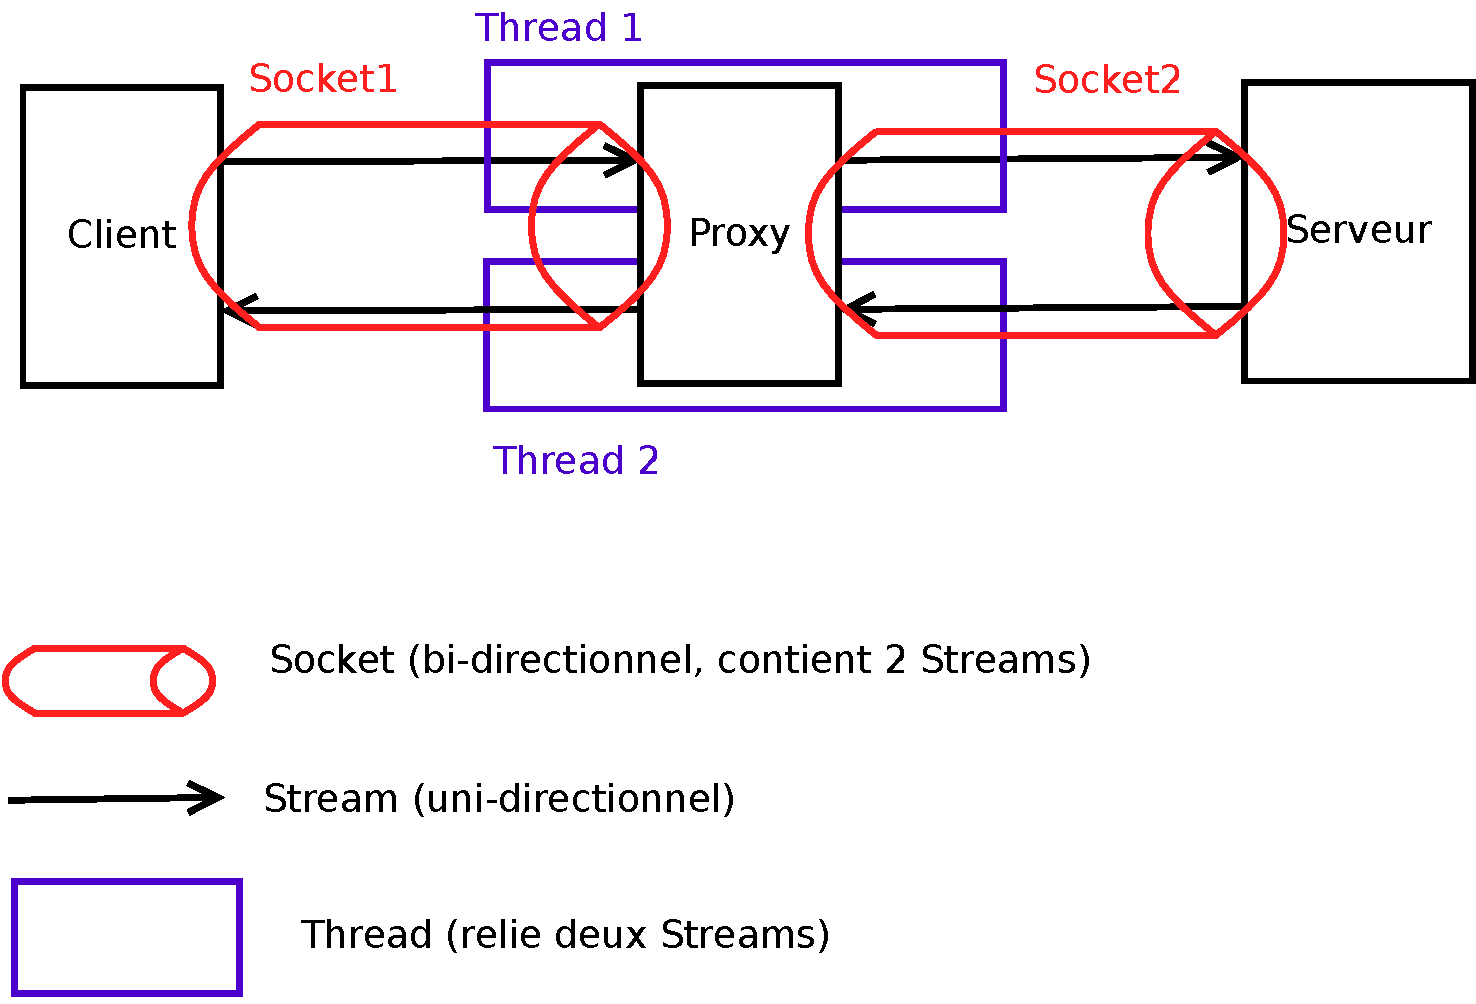
\includegraphics[width=\textwidth]{images/thread.pdf}
	\end{frame} 

	
	\begin{frame}
		\frametitle{Sockets}	
		\framesubtitle{Types de sockets dans Java}
		\begin{itemize}
			\item Socket
			\item SSLSocket
			\item ServerSocket
			\item SSLServerSocket
		\end{itemize}
	\end{frame} 
	
	\begin{frame}
		\frametitle{Sockets}	
		\framesubtitle{Utilisation en HTTP}
		\begin{itemize}
			\item Entre Client et Proxy
			\begin{itemize}
				\item Nécessité d'une ServerSocket en écoute.
				\item Création d'une Socket à la suite d'une connexion.
			\end{itemize}
			\item Entre Serveur et Proxy
			\begin{itemize}
				\item Récupération de l'ip et du port du serveur.
				\item Création d'une Socket pour se connecter au serveur.
			\end{itemize}
		\end{itemize}
	\end{frame}

	\begin{frame}
		\frametitle{Sockets}	
		\framesubtitle{Utilisation en HTTPS}
		\begin{itemize}
			\item Entre Client et Proxy
			\begin{itemize}
				\item Même déroulement que pour HTTP au début.
				\item Transformation de la Socket en SSLSocket en utilisant un Keystore pour trouver le certificat adéquat.
			\end{itemize}
			\item Entre Serveur et Proxy
			\begin{itemize}
				\item Même déroulement que pour HTTP au début.
				\item Création d'une SSLSocket pour se connecter au serveur et récupérer son certificat.
			\end{itemize}
		\end{itemize}
	\end{frame}

	\begin{frame}
		\frametitle{Keystore}
		\framesubtitle{Création}
		\begin{itemize}
			\item Sert à gérer les certificats pour les connexions sécurisées.
			\item Contient les autorités de certification reconnues par Java.
			\item Contient également notre autorité qui signera les faux certificats.
		\end{itemize}
	\end{frame} 
	
 		\begin{frame}
		\frametitle{Keystore}
		\framesubtitle{Utilisation}
		\begin{itemize}
			\item Génération d'un certificat semblable à celui du serveur.
			\item Création d'un fichier PKCS\#12 contenant ce certificat.
			\item Création d'un nouveau KeyStore à partir de ce PKCS\#12.
		\end{itemize}				
	\end{frame}
	
	\begin{frame}
		\frametitle{Journalisation}
		\begin{itemize}
			\item Récupération du trafic en clair dans un fichier.
			\item Précision sur l'heure et le sens de l'envoi.
		\end{itemize}				
	\end{frame} 
	
	